% -*- TeX:de -*-
\NeedsTeXFormat{LaTeX2e}
\documentclass[12pt,a4paper]{article}
\usepackage[german]{babel} % german text
\usepackage[DIV12]{typearea} % size of printable area
\usepackage[T1]{fontenc} % font encoding
%\usepackage[latin1]{inputenc} % most likely on Windows
\usepackage[utf8]{inputenc} % probably on Linux
\usepackage{multicol}

% PLOTTING
\usepackage{pgfplots} 
\usepackage{pgfplotstable}
\usepackage{url}
\usepackage{graphicx} % to include images
\usepackage{tikz}
\usepackage{subfigure} % for creating subfigures
\usepackage{amsmath} % a bunch of symbols
\usepackage{amssymb} % even more symbols
\usepackage{booktabs} % pretty tables
\usepackage{makecell} % multi row table heading

% a floating environment for circuits
\usepackage{float}
\usepackage{caption}

%\newfloat{circuit}{tbph}{circuits}
%\floatname{circuit}{Schaltplan}

% a floating environment for diagrams
%\newfloat{diagram}{tbph}{diagrams}
%\floatname{diagram}{Diagramm}

\selectlanguage{german} % use german

\begin{document}








%%%% TO DO
%
% - - Shorty:
%

% - - Patrick
%




%%%%%%% DECKBLATT %%%%%%%
\thispagestyle{empty}
			\begin{center}
			\Large{Fakultät für Physik}\\
			\end{center}
\begin{verbatim}


\end{verbatim}
							%Eintrag des Wintersemesters
			\begin{center}
			\textbf{\LARGE WS 2013/14}
			\end{center}
\begin{verbatim}


\end{verbatim}
			\begin{center}
			\textbf{\LARGE{Physikalisches Praktikum\\ für das Bachelorstudium}}
			\end{center}
\begin{verbatim}




\end{verbatim}

			\begin{center}
			\textbf{\LARGE{PROTOKOLL}}
			\end{center}
			
\begin{verbatim}





\end{verbatim}

			\begin{flushleft}
			\textbf{\Large{Experiment (Nr., Titel):}}\\
							%Experiment Nr. und Titel statt den Punkten eintragen
			\LARGE{PW5 Gasthermometer, Adiabatenkoeffizienten, Dampfdichte}	
			\end{flushleft}

\begin{verbatim}

\end{verbatim}	
							%Eintragen des Abgabedatums, oder des Erstelldatums des Protokolls
			\begin{flushleft}
			\textbf{\Large{Datum:}} \Large{07.11.2013}
			\end{flushleft}
			
\begin{verbatim}
\end{verbatim}
							%Namen der Protokollschreiber
		\begin{flushleft}
			\textbf{\Large{Namen:}} \Large{Patrick Braun, Johannes Kurz}
			\end{flushleft}

\begin{verbatim}


\end{verbatim}
							%Kurstag und Gruppennummer, zb. Fr/5
			\begin{flushleft}
			\textbf{\Large{Kurstag/Gruppe:}} \Large{DO/2}
			\end{flushleft}

\begin{verbatim}



\end{verbatim}
							%Name des Betreuers, das Praktikum betreute.
			\begin{flushleft}
			\LARGE{\textbf{Betreuer:}}	\Large{ Franz Sachslehner }	
			\end{flushleft}

%%%%%%% DECKBLATT ENDE %%%%%%%
\pagebreak
\setlength{\columnsep}{20pt}
\begin{multicols}{2}

%%%%%%%%%%%%%%%%%%%%%%%%%%%%%%%%%%%%
\section{Gasthermometer}

\begin{figure}[H]
	\centering
	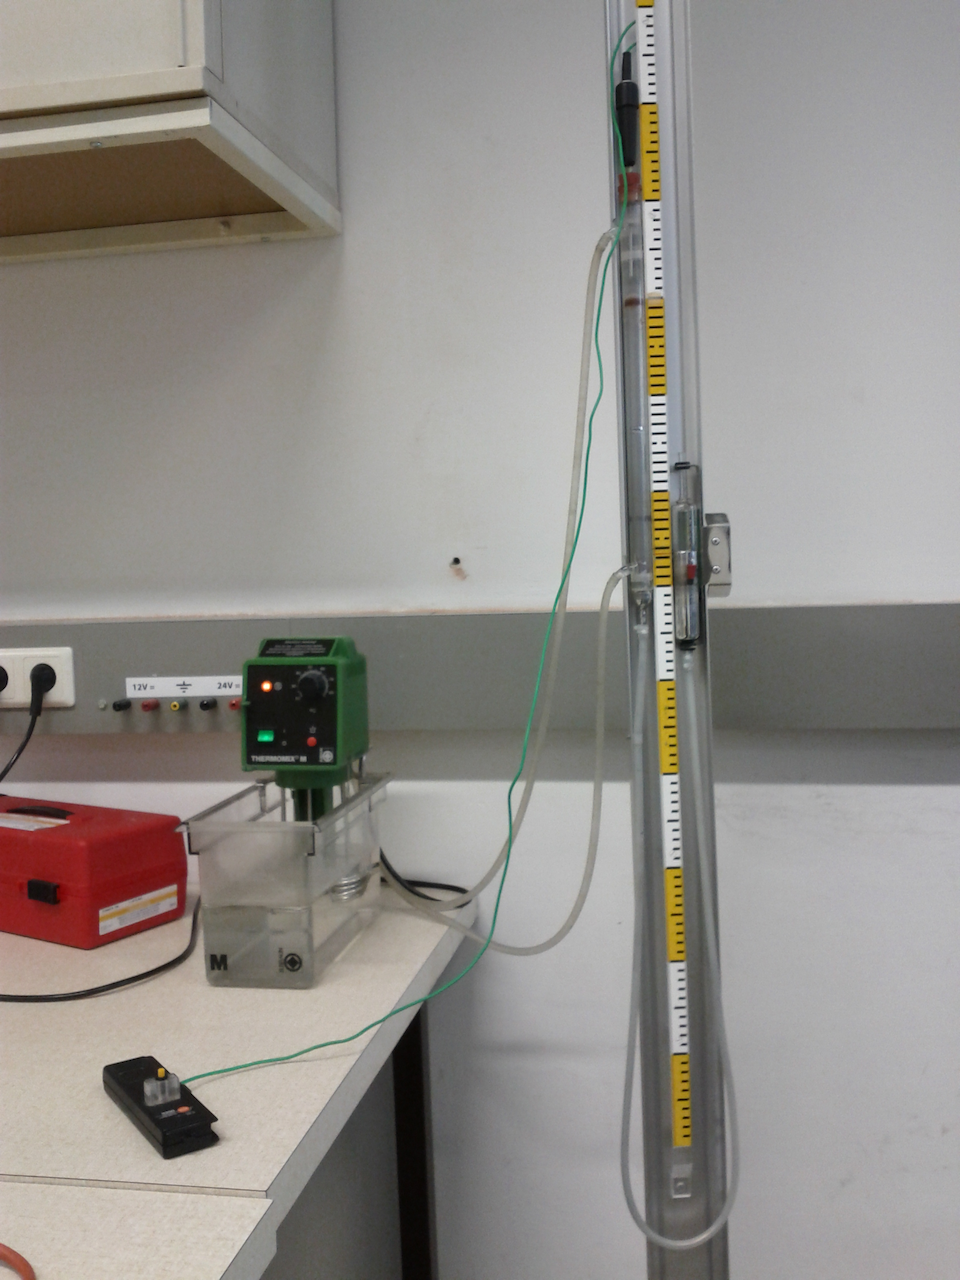
\includegraphics[scale=0.22]{./figure/gas_therm_aufbau.png}
	\caption{Versuchsaufbau mit Heizgerät und Thermometer}
	\label{fig:gas_therm_aufbau}
\end{figure}

%Equipment:
%\begin{itemize}
%	\item[-] Testoterm Sekundenthermometer (9200)
%	\item[-] Halterung mit Quecksilbergefüllten Röhren (siehe Abb. \ref{fig:gas_therm_aufbau} rechts)
%	\item[-] Heizgerät Thermomix B.Braun
%\end{itemize}

\subsection{Messwerte und Ergebnisse}
Außendruck: 993mBar\\


\subsection{Diskussion}




%%%%%%%%%%%%%%%%%%%%%%%%%%%%%%%%%%%%
\section{Adiabatenkoeffizient der Luft}
In diesem Experiment bestimmen wir den Adiabatenkoeffizienten der Luft. Wird ein Gas komprimiert ohne das Wärme entweichen kann, steigt der Druck stärker an als wenn die Wärme entweichen kann. Im Normalfall (isotherm) entspricht der Druck
$$p = \frac{C}{V}$$
wobei C eine Konstante ist.
Im adiabatischen Fall, den wir Näherungsweise durch Luft erhalten welche ihren Druck in kurzen Intervallen ändert, entspricht der Druck:
$$p = \frac{C}{V^\kappa}$$
Es gibt in der Theorie einen Zusammenhang zwischen dem Koeffizienten $\kappa$ und den Freiheitsgraden der Moleküle im Gas. Bei Luft haben wir 6 Freiheitsgrade (3 Raumdimensionen, 3 Rotationsachsen) wobei die Eigendrehung entlang der Achse quer durch das Molekül kaum bis keinen Beitrag zu unserem Problem leistet und daher vernachlässigt wird. Mit 5 Freiheitsgraden ergibt sich ein erwarteter Wert von
$$\kappa = \frac{f+2}{f} = \frac{7}{5} = 1.4$$
Um diesen Wert Experimentell zu bestimmen verwenden wir ein 10L Gefäß und einen Gummi Blasebalg um eine Metallkugel in Schwingung zu versetzen. Der Aufbau ist in \ref{fig:adiabatenkoeffizienten_aufbau} ersichtlich.
\begin{figure}[H]
	\centering
	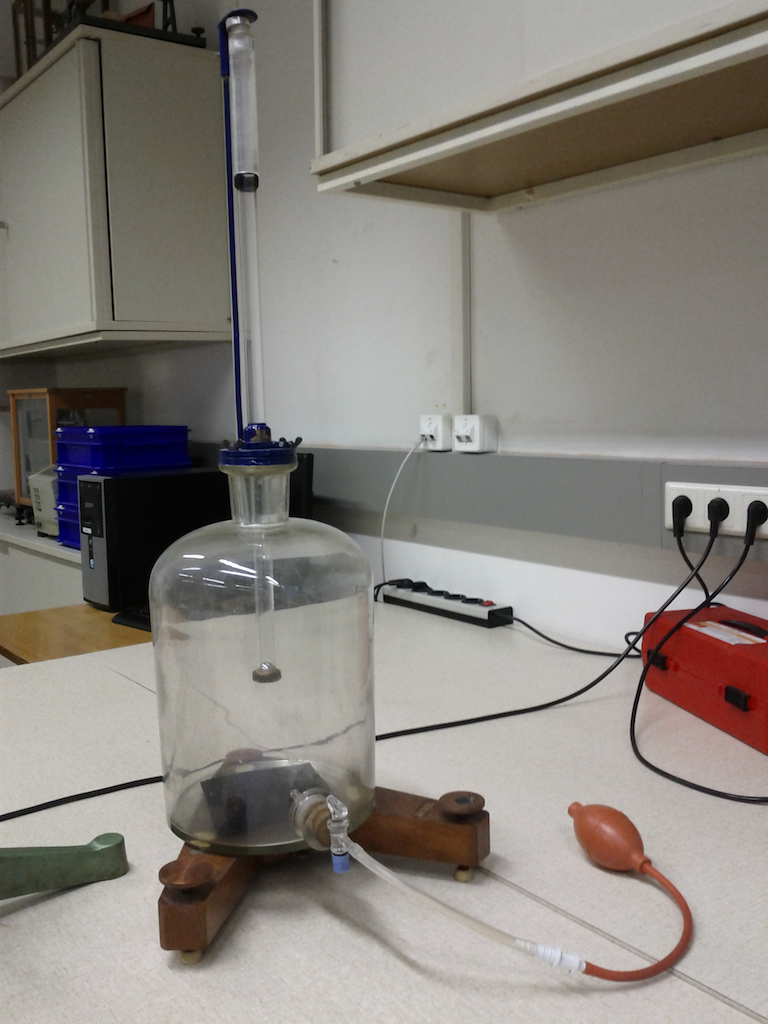
\includegraphics[scale=0.25]{./figure/koeffizient.png}
	\caption{Versuchsaufbau zur Ermittlung des Adiabatenkoeffizienten der Luft}
	\label{fig:adiabatenkoeffizienten_aufbau}
\end{figure}
\noindent
Nach der Herleitung (aus 3.1.3 [1]) erhalten wir folgende Formal für $\kappa$:
$$\kappa = \left(\frac{2\pi}{T}\right)^2  \frac{m V_0}{q^2  p}$$
T... Gemittelte Periodendauer der gemessenen Schwingungen\\
m... Masse der Kugel\\
$V_0$... Volumen des Behälters\\
q... Querschnittsfläche der Röhre in der sich die Kugel bewegt\\
p... Druck\\
\\
Den Druck lässt sich errechnen durch:
$$p = p_0 + \frac{m g}{q}$$
$p_0$... Außendruck (Luftdruck)\\
g... Erdbeschleunigung\\
Mit den angegebenen Werten aus [1] 3.3.1, den gemessenen Zeiten für T und der gemessenen Masse der Kugel errechnen wir im folgenden Abschnitt $\kappa$.
%Equipment:
%\begin{itemize}
%	\item[-] Stoppuhr
%	\item[-] Versuchsaufbau mit Pumpe und Metallkugel in Röhre
%\end{itemize}
%
\subsection{Messwerte und Ergebnisse}

Masse Kugel (Zwei Messungen, mit Papier und Papier allein):\\
Kugel mit Papier: $(18,638 \pm 0.005)g$\\
Papier allein: $(1,810 \pm 0.005)g$\\
$(16.828 \pm 0.008)g$ \\
%Zwei Messungen, Kugel mit Papier, nur Papier => zwei mal Messfehler.\\
Werte von 3 mal 6 Messungen:
\begin{figure}[H]
	\centering
	\pgfplotstabletypeset[
			columns={T1,T2,T3},
			col sep=&,
			columns/T1/.style={column name=$T_1[s]$, precision=2, zerofill}, %\makecell{Line 1\\Line 2}
			columns/T2/.style={column name=$T_2[s]$, precision=2, zerofill},
			columns/T3/.style={column name=$T_3[s]$, precision=2, zerofill},
			every head row/.style={before row=\hline,after row=\hline\hline},
			every last row/.style={after row=\hline},
			every first column/.style={
								column type/.add={|}{}
							        },
			every last column/.style={
								column type/.add={}{|}
								}
			]{
			T1 & T2 & T3
			5.35 & 5.35 & 5.40
			5.49 & 5.36 & 5.37
			5.40 & 5.39 & 5.35
			5.37 & 5.49 & 5.41
			5.43 & 5.33 & 5.46
			5.31 & 5.46 & 5.44
			}
	\caption{Periodendauer nach 5 Schwingungen}
	\label{fig:adiabaten_periode_messung}
\end{figure}
\noindent
Mean: 5,39778 s\\
STABW: 0,05418s\\
Standard Error of mean: 0,01277s\\

\subsection{Diskussion}
Da der Fehler von 0.005g zweimal in die Messung eingeht steigert der Fehler sich aufgerundet auf 0.008.
\ref{fig:adiabaten_periode_messung}


%%%%%% Dampfdichtebestimmung %%%%%%%%

\section{Dampfdichtebestimmung}



\subsection{Messwerte und Ergebnisse}



\subsection{Diskussion}



\section{Quellen}
[1] Leitfaden, \url{http://www.univie.ac.at/anfpra/neu1/pw/pw5/PW5_PL1.pdf}\\

\end{multicols}
\end{document}